%   File: FirstAndTen.tex
% Author: Adam Leeper
%------------------------------------------------------------------------------
%\\[0.45pc]
\providecommand{\isolatedBuild}[1]{#1}% Fallback definition to build normally.
\isolatedBuild{
  \documentclass[11pt,letterpaper]{book}
  %\documentclass[11pt,letterpaper]{book}

% aleeper: I think these are needed for Paul's macros?
\usepackage{epsfig}
\usepackage{epstopdf}

%\makeatletter
%\typeout{The import path is \import@path}
%\makeatother

\usepackage{import}

\subimport{./}{packagesMitiguy.sty}
\subimport{./}{macrosMitiguy.tex}
\subimport{./}{PageStylesMitiguy.tex}
\subimport{./}{macrosLeeper.tex}
   % Found via TEXINPUTS environment variable.
  \isolatedBuildHeader{Vector Equations and Geometry}
                      {Cameras and Robotics in the NFL}
}
%%%
%%%
%%%
%%%%%%%%%%%%%%%%%%%%%%%%%%%%%%%%%%%%%%%%%%%%%%%%%%%%%%%%%%%
%
\begin{minipage}[t]{0.7\linewidth}
  The 1st and Ten Graphics System is used to  show a virtual yellow line on
  video footage of football games.The system continuously measures the position
  and orientation of the camera relative to the the field. Hence, position
  information from the field can be converted into the frame of the camera for
  overlaying on the video in real-time, even as the camera rotates.
  %When an operator clicks on the image, the click location is converted into a
  %position on the field.
  \\[0.45pc]
  Let the field be a rigid frame \basis{N} with orthogonal unit
  vectors ~\uvecBasisxyz{n} oriented as shown.
  Let point \origin{N} be fixed in \basis{N} at zero height above the field.
  Assume the field lies in the ~\uvecxy{n} plane.
  %
  \\[0.45pc]
  Let the camera body be a rigid frame \basis{B} with orthogonal
  unit vectors ~\uvecBasisxyz{b} and a point \origin{B} fixed in \basis{B}.
  Assume the position vector from \origin{N} to \origin{B} is known to be
  $\posvec{\origin{N}}{\origin{B}} \equals (\SI{50}{yards})~\uvecx{n}
  \plus (\SI{20}{yards})~\uvecz{n}$.
  %
  \\[0.45pc] Finally, let the football be identified as point $Q$.
\end{minipage}
\hfill
\begin{minipage}[t]{0.27\linewidth}
  \vspace{-0.5pc}
  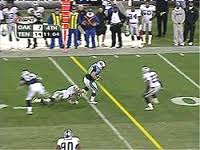
\includegraphics[width=\linewidth]{firstAndTen.jpg}
\end{minipage}
\\[0.2pc]
%
\begin{enumerate}
  \item
    %\\[0.5pc]
    \begin{minipage}[t]{0.6\linewidth}
      When the football is lying on the field, the operator clicks on the
      football in the video. Assume the click is converted into a direction
      vector pointing to $Q$ from \origin{B} as
      $~\uvecWithHat{u}^{Q \division \origin{B}} \equals 1~\uvecx{b}$.
      \\[0.5pc]
      Find a \textbf{system of \boldUnderlineDarkRed{scalar} equations} that can be
      used to solve for the \underline{~\uvecx{n} and ~\uvecy{n} measures} of the
      football's position from \origin{N}. The rotation table will be formed later; for
      now you may leave unknown dot-products un-evaluated
      (such as $~\uvecx{b} \cdot ~\uvecx{n}$).
      \\[0.5pc]
      To do this, it may help to:
      \begin{itemize}
        \item Introduce \boldDarkRed{unknown} measures for $Q$'s position
          from \origin{N} to help you express \posvec{\origin{N}}{Q}.
        \item Write \posvec{\origin{B}}{Q} as an \boldDarkRed{unknown} multiple of
          $~\uvecWithHat{u}^{Q \division \origin{B}}$.
        \item Write a \boldDarkRed{vector loop} equation.
      \end{itemize}
    \end{minipage}
    \hfill
    \begin{minipage}[t]{0.44\linewidth}
      \minipageTopAnchor
      %\vspace*{-1cm}
      \begin{center}
        \includegraphicsAB[width=0.66\linewidth]
          {football-solution.png}
          {football.png}
      \end{center}
    \end{minipage}
    \Solution{}{0.99\linewidth}{
      \begin{minipage}{0.65\linewidth}
        \begin{tabular}{@{ }l@{}r@{ \equals[\;] }ll}
          & \posvec{\origin{N}}{Q}& $x~\uvecx{n} \plus y~\uvecy{n} \plus 0~\uvecz{n}$
            \\[1.0pc]
            & \posvec{\origin{N}}{\origin{B}}& $50~\uvecx{n} \plus 0~\uvecy{n} \plus 20~\uvecz{n}$
            \\[1.0pc]
            & \posvec{\origin{B}}{Q}& $\lambda~\uvecx{b}$
            \\[1.0pc]
            Loop:& \posvec{\origin{N}}{Q}& \posvec{\origin{N}}{\origin{B}}\plus\posvec{\origin{B}}{Q}
            \\[1.0pc]
            & $x~\uvecx{n} \plus y~\uvecy{n}$& $50~\uvecx{n} \plus
            20~\uvecz{n} \plus\lambda~\uvecx{b}$
            \\[1.0pc]
            dot w/ ~\uvecx{n}:& x & $ 50 \plus \lambda ~\uvecx{b} \DotProduct ~\uvecx{n} $
            \\[1.0pc]
            dot w/ ~\uvecy{n}:& y & $ 0 \plus \lambda ~\uvecx{b} \DotProduct ~\uvecy{n} $
            \\[1.0pc]
            dot w/ ~\uvecz{n}:& 0 & $ 20 \plus \lambda ~\uvecx{b} \DotProduct ~\uvecz{n} $
        \end{tabular}
        \\[0.45pc]
        The 3 equations above form a scalar system of equations with 3 unknowns.
      \end{minipage}
    }
  %%%%%%%%%%%%%%%%%%%%%%%%%%%%%%%%%%%%%%%%%%%%%%%%%
  \clearpage
  \item
  %\hspace*{0pt}%\textbf{( 12 pts )}
  %\\[-2.7pc]
    \begin{minipage}[t]{0.53\columnwidth}
      The camera body is mounted on a pan-tilt mechanism; the ``pan" part
      lets the camera rotate ``left-and-right" and the ``tilt" part lets
      the camera rotate ``up-and-down".
      \\[1.0pc]
      Let the ``pan" portion of the mechanism be a rigid frame \basis{A}
      with orthogonal unit vectors ~\uvecxyz{a}. Frame \basis{A} is initially
      aligned with \basis{N} but is then rotated with $\plus~\uvecz{n}$ sense
      by an angle $\theta$.
      (Hint: $\theta$ is the angle between ~\uvecy{n} and ~\uvecy{a}.)
      \\[1.0pc]
      The ``tilt" portion of the mechanism can be assumed to be the same
      as the camera body frame \basis{B}, which is initially aligned with
      \basis{A} but is then rotated with $\plus~\uvecy{a}$ sense by an angle
      $\phi$. (Hint: $\phi$ is the angle between
      ~\uvecx{a} and ~\uvecx{b}.)
      \\[1.0pc]
      Please \textbf{\underline{write two rotation tables}}: one relating
      \basis{N} and \basis{A} and one relating \basis{A} and \basis{B}.
      \\[0.25pc]
      Then \textbf{\underline{explain}} how to obtain the rotation
      table relating frame \basis{N} and \basis{B}
      (don't actually compute it).
    \end{minipage}
    \hfill
    \begin{minipage}[t]{0.37\columnwidth}
      \flushright
      \vspace*{0pt}
      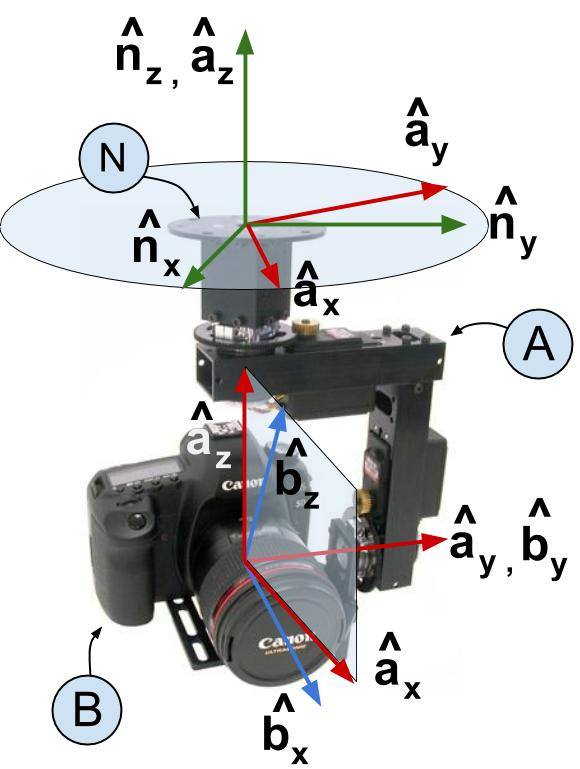
\includegraphics[width=7cm]{camera_pan_tilt.jpg}
    \end{minipage}
    \Solution{}{0.99\linewidth}{
      \begin{minipage}{0.34\linewidth}
        \minipageTopAnchor
        \center
        \rotationTable{N}{A}
          {\cos\theta}{-\sin\theta}{0}
          {\sin\theta}{\cos\theta}{0}
          {0} {0} {1}
        \\[1.0pc]
      \end{minipage}
      \begin{minipage}{0.34\linewidth}
        \minipageTopAnchor
        \center
        \rotationTable{A}{B}
          {\cos\phi}{0}{\sin\phi}
          {0} {1} {0}
          {-\sin\phi}{0}{\cos\phi}
        \\[1.0pc]
      \end{minipage}
      \\[0.45pc]
      To get \dircos{N}{B}, treat \dircos{N}{A} and
      \dircos{A}{B} as matrices, and perform the matrix
      mulitplication:
      \center
      \dircos{N}{B} \equals \dircos{N}{A}
      \mult[] \dircos{A}{B}
    }
  %%%%%%%%%%%%%%%%%%%%%%%%%%%%%%%%%%%%%%%
  \clearpage
  \item %\textbf{( 10 pts )}
    To save you time, you are given the resulting rotation table
    relating frame \basis{N} and \basis{B}
    \\[0.5pc]
    \rotationTable{N}{B}
      {\cos(\theta)\cos(\phi)}{-\sin(\theta)}{\cos(\theta)\sin(\phi)}
      {\sin(\theta)\cos(\phi)}{\cos(\theta)}{\sin(\theta)\sin(\phi)}
      {-\sin(\phi)}{0}{\cos(\phi)}
    \\[1.0pc]
    Use your result from part (a) to \textbf{\underline{actually solve for
    the ~\uvecx{n} and ~\uvecy{n} measures}} of the football's position from
    \origin{N} when $\theta \equals \degrees{30}$ and $\phi \equals \degrees{45}$.
    (I want numbers with appropriate units.)
    \\[1.0pc]
    \Solution{}{0.99\linewidth}{
      \begin{minipage}{0.65\linewidth}
        \minipageTopAnchor
        \center
        \begin{tabular}{@{ }l@{}r@{ \equals[\;] }lll}
          $\lambda$ \equals& \fracDisplaystyle{\minus20}
          {~\uvecx{b}\cdot~\uvecz{n}}
          & $\fracDisplaystyle{\minus20}{\minus\sin{\degrees{45}}}$
          & \equals $\fracDisplaystyle{20}{\sqrt{2}/2}$\equals
          & 20$\sqrt{2}$
          \\[1.0pc]
          y \equals& $\lambda ~\uvecx{b}\cdot~\uvecz{n}$&
          (20$\sqrt{2})\sin(\degrees{30})\cos(\degrees{45})$
          \\[1.0pc]
          && 20$\sqrt{2}\left(\fracDisplaystyle{1}{2}\right)
          \left(\fracDisplaystyle{\sqrt{2}}{2}\right)$
          \\[1.0pc]
          && \SI{10}{yards}
          \\[1.0pc]
          x \equals& 50\plus$\lambda~\uvecx{b}\cdot~\uvecx{n}$
          & 50\plus20$\sqrt{2}\cos(\degrees{30})\cos(\degrees{45})$
          \\[1.0pc]
          && 50\plus20$\sqrt{2}\left(\fracDisplaystyle{\sqrt{3}}{2}\right)
          \left(\fracDisplaystyle{\sqrt{2}}{2}\right)$
          \\[1.0pc]
          && 50\plus10$\sqrt{3}$
          \\[1.0pc]
          && \SI{67.3}{yards}
          \\[1.0pc]
          \posvec{\origin{N}}{Q}&& \SI{67.3}{yards} ~\uvecx{n} \plus \SI{10}{yards} ~\uvecy{n}
        \end{tabular}
      \end{minipage}
      \\[0.45pc]
    }
  %
  \item %\textbf{( 5 pts )}
    For the actual camera \textit{optical} frame \basis{C}, the convention
    in the camera industry is to assign orthogonal unit vectors ~\uvecx{c} to
    the right, ~\uvecy{c} down, and ~\uvecz{c} forward. However, a roboticist
    created the pan-tilt mechanism and assigned the frames
    \basis{A} and \basis{B}.
    From the figure, please \textbf{\underline{write a rotation table}} relating
    frame \basis{B} and \basis{C}. (There are no angles involved).
    \\[1.0pc]
  \todo{NEED TO ADD FIGURE}
\end{enumerate}
%
\isolatedBuildFooter
